\section{\I {The population section: model structure and the population dynamics}\label{sec:Population}}

The command and subcommand syntax for the estimation section is given in Section \ref{syntax:Population}.

\subsection{Introduction}

This section\index{Population section} shows how to specify a model for the population dynamics. It describes the model time and age scope, the population processes used (e.g., recruitment, ageing, migration, and mortality), the selectivity ogives, and how to set values for their associated parameters, or starting values if they are going to be estimated.

The basic structure of the population is defined in terms of its partitions and the succession of processes that act on them throughout a year. \CNAME\ assumes an annual cycle, i.e., rates like natural mortality are assumed to be for a year. To place certain processes or observations (e.g., a research survey) into the right part of the year, the year can be divided into one or more time steps, and each time step needs  at least one process. Each time step can represent a specific period of the calendar year, or it can be an abstract sequence of events. Certain processes like natural mortality and growth can have a proportion of the effects of the process assigned to different time steps to crudely mimic seasonal effects, or fisheries that occur in short periods of the year, as well as place a survey within the year relative to the proportion of annual natural mortality that has occurred (see Section \ref{sec:DerivedQuantity}).

The \emph{state} is the current status of the population at any given time and it can change one or more times during the year. The state object must contain sufficient information to determine how the population changes over time, given a model and a complete set of parameters. The partition is key to the state, but it has no "memory". Thus, other information must also be kept, such as the mature biomass from a previous year or time step to calculate the recruit numbers into the first age class via the spawner-recruitment relationship. Quantities like mature biomass are defined as \emph{derived variables} and are calculated for each year of the model. However, the \emph{derived variables} record only summary information from the partition at a specified time step and year.

Processes can change the partition and, for example, include recruitment, natural mortality, fishing mortality, ageing, migration, and maturation. These processes are repeated for each year of the model.

The specification and ordering of processes in multiple time steps can be used to represent complex dynamics, with the intermingling of multiple species and stocks, migration patterns occurring over multiple areas, and/or multiple sources of anthropogenic impacts using a range of methods which cover different areas and times.

However, the complexity of a stock structure definition is constrained by the available data. It is challenging to use a complex structure to model a population when there are no observations to support that structure.  For information on how to define categories and use the shorthand syntax see Section \ref{sec:ShorthandSyntax}.

Topics covered are:

\begin{itemize}
	\item The model scope, such as the ages covered, the years over which the model runs, and the end year for projections (Section~\ref{sec:Model});
    \item Linking processes, such as growth, to each category;
    \item The number of time steps and the processes that are applied in each time step\index{Annual cycle} (Section~\ref{sec:TimeStep});
    \item The specification of and the parameters for the population processes: processes that add or remove individuals from a partition, or shift individuals between ages and categories in a partition;
    \item The initialisation process: the state of the partition at the start of the first year\index{Initialisation}\index{Model ! initialisation};
   \item Defining selectivity ogives and linking them to observations;
   \item The parameters: their definitions, initial values, prior distributions, and other characteristics; and
   \item Derived quantities, e.g., mature biomass, to include in density-dependent processes such as the spawner-recruit relationship
\end{itemize}

\subsection{\I{Model scope and structure}}\label{sec:Model}

The model needs scoping for ages and year covered. This is done in the \command{model} command block.

Each \CNAME\ model requires:

\begin{itemize}
\item The minimum and maximum population ages
\item Whether the maximum age is a plus group
\item The start and final year
\item The names of all of the categories
\end{itemize}

The ages used starts at the minimum age through to the maximum age in steps of one. The model is run from the start year through to the final year. It can also be run past the final year to project the state of the population through the final projection year.

An example of how to specify a potential model with two categories is outlined below;  the \command{model} and \command{categories} blocks are:

{\small{\begin{verbatim}
		@model
		start_year 1981
		final_year 2000
		projection_final_year 2010
		base_weight_units     tonnes
		min_age    1
		max_age   20
		age_plus_group        true
		initialisation_phases Equilibrium_phase
		time_steps            step1 step2 step3

		@categories
		format      sex
		names       male female
		age_lengths male_growth female_growth  # labels for growth blocks
\end{verbatim}}}

This model runs for 20 years, starting in 1981, and will do a projection over 10 years for a population with ages from  1 through 20, with age 20 being a plus-group. Each year is divided into three time-steps. The categories are male and female (i.e., there is one category factor, labelled \textit{sex}) and each category has an age-length relationship.

Whist \CNAME\ generally uses generic formulation, it does have some specific population concepts, in this case, growth which can vary for each category. Additionally, there is a  length-weight characteristic which is specified in the age-length blocks, which in this example are command blocks starting with \command{age\_size male\_growth} and \command{age\_size female\_growth} that are placed elsewhere in the input files (not shown).

\CNAME\ allows categories of the partition to exist for a subset of years of a model. This feature enables more efficient computations when models contain categories that do not persist over all model years. A model may define one-off processes that transition individuals from one category into another in a subset of the model initialisation phases or years (e.g., tagging events). Excluding categories for certain years can be more efficient as \CNAME\ will not initialise these categories or apply processes to categories in years or time steps in which they do not exist.

The structure of the partition is defined in a configuration block with the \command{categories} block (Section \ref{sec:Model}).

Derived quantities are an important component of the state object. An example of a derived quantity is spawning stock biomass (SSB; the biomass of [female] spawning fish calculated at the mid point of the spawning season). \CNAME\ calculates derived quantities using the command \command{derived\_quantity}, required for some processes. In fisheries stock assessment models, a recruitment process which includes a stock-recruitment relationship requires the definition of a derived quantity that specifies the mid-season spawning stock biomass. See Section \ref{sec:DerivedQuantity} for more details.

\subsubsection{\I{The implicit annual cycle}}\label{sec:TimeStep}

There is an implicit annual cycle that orders the sequence of processes within the year, but there is no command block as such. The implementation is by ordering processes within the time-steps. This sequence is repeated for every year. Time steps are used to break the year into separate components and allow observations to be associated with specific time periods and processes. Any number of processes can occur within each time step, in any order, although there are restrictions for mortality-based processes (see Section~\ref{sec:Process-Mortality}); processes can occur multiple times within each time step. Time steps are not implemented during the initialisation phases (effectively there is only one initialisation time step), and the annual cycle in the initialisation phases can be different from the annual cycle specified for the model years (\ref{sec:Initialisation}).

Figure \ref{Fig:annual} shows an example of the annual cycle using three time-steps.

\begin{figure}[H]
	\centering
	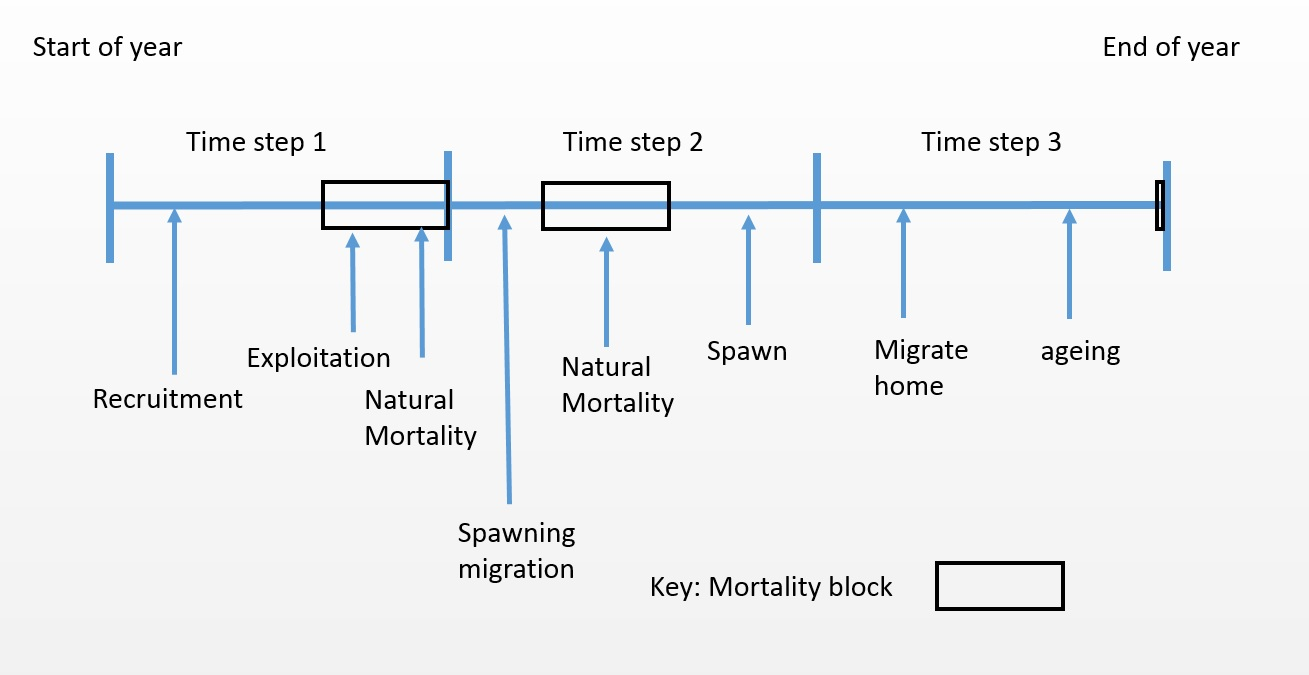
\includegraphics[scale=0.5]{Figures/annual_cycle.jpg}
	\caption{A example sequence for an annual cycle.}\label{Fig:annual}
\end{figure}

This would be specified using \command{time\_step} block:

{\small{\begin{verbatim}
@model
time_steps step1 step2 step3
\end{verbatim}}}

This gives the order and labels for each time step, i.e., 3. Processes are sequenced using order within the \command{time\_step} block:

{\small{\begin{verbatim}
@time_step step1
processes Recruitment Fishing

@time_step step2
processes Spawn_migration Fishing

@time_step step3
processes Home_migration Ageing
\end{verbatim}}}

The \emph{Recruitment}, \emph{Fishing}, \emph{Spawn\_migration}, \emph{Home\_migration} and \emph{Ageing} are all labels of command blocks that defines a process (see Section \ref{sec:Process} for the list of available processes). The order that the  processes are executed is in the same order as specified. The process \emph{Fishing} could be the process type \texttt{Instantaneous\_Mortality} (Section 
\ifAgeBased
\ref{sec:Process-MortalityInstantaneous}
\else
\ref{sec:Process-Length-MortalityInstantaneous}
\fi
) which takes natural mortality as a parameter as well as specifying the catches in the time-steps, so it is possible to have all catch taken in time-step \emph{step1} with some natural mortality, and no fishing in time-step \emph{step2} where the rest of the natural mortality occurs.

Although the process \emph{Spawn} represents a biological process, spawning, in the \CNAME\ model it is the time that the spawning stock biomass ($SSB$) is calculated since this is needed to calculate recruitment if there is a spawner-recruitment relationship. A related concept is maturity which can be in the partition, so there needs to be a process to transfer immature fish into the mature category, but it is only indirectly related to spawning. Hence, in modelling, spawning is not a process that affects the partition directly, but it the time to calculate the $SSB$ which must be defined as a derived quantity (from the partition). Hence, \emph{Spawn} is located in Figure \ref{Fig:annual}.

To calculate the $SSB$ a \command{derived\_quantity} command block is needed in which the "timing" of the $SSB$ calculation in terms of which time-step and the proportion of natural mortality within it is specified (\ref{sec:DerivedQuantity}).

\subsubsection{\I{The initialisation phases}}\label{sec:Initialisation}

Initialisation is the process of determining the model starting state at the start of the first year (\texttt{Start\_year}. The initial state can be equilibrium/steady state or some other initial state for the model (e.g., exploited), prior to the start year of the model.

There are multiple options for partition initialisation in \CNAME, including

\begin{itemize}
	\item Iterative: run the model for a specified number of years to get the converged state.
	\item Derived: Use the analytical solution (i.e., faster than iterative) for the initial state, but it does not work with some processes (e.g., density-dependent migration)
	\item Cinitial: Estimate the initial partition's numbers-at-age
	\item state\_category\_by\_age: specify the partition's numbers-at-age
\end{itemize}

Initialisation definitions start with specifying the initialisation label in the \command{model} command block followed by a \command{initialisation\_phase} command block specifying the type and other settings:

{\small{\begin{verbatim}
@model
...     # other subcommands
initialisation_phase int_label

@initialisation_phase int_label
type iterative  #choose one from the list above
...             # specify option values

\end{verbatim}}}

If needed, the processes used and their order in the initialisation are those specified in the annual cycle, but these can by changed by either excluding some processes or including others by using the  \texttt{exclude\_processes} or  \texttt{insert\_processes} subcommands in the \textit{initialisation\_phase} command blocks,

{\small{\begin{verbatim}

@initialisation_phase int_label
type iterative
exclude_processes Fishing
insert_processes step1(recruitment)=initialFishing
            # format: <step>(<insert before process label>)=<new block label>
...         # specify option values

\end{verbatim}}}

where \textit{Fishing} is the normal fishing process which defines natural mortality so when excluded, initialisation can use another value that incorporates some unrecorded fishing before the start of the assessment period by setting natural mortality to a higher value in the process \textit{initialFishing}. The place to insert \textit{initialFishing} is in the time-step labelled \textit{step1} before the process \textit{recruitment} which must be in that time-step (process label is enclosed in brackets). To insert at the end of the time-step use \textit{()}, e.g. \textit{step1()=initialFishing}.

For age-based models the most common type of initialisation phase to define an equilibrium age structure is \subcommand{derived}, whereas for length-based models the only type available is \subcommand{iterative}. Additional initialisation phases can be included by sequencing other phases one after another

{\small{\begin{verbatim}
@model
...     # other subcommands
initialisation_phase int_label int_label2


@initialisation_phase int_label
type derived    #choose one from the list above
...             # specify option values

@initialisation_phase int_label2
type iterative    #choose one from the list above
...             # specify option values

\end{verbatim}}}

which may be faster overall since fewer iterations may be required used in the second phase. The order of applying each initialisation is that given in the \command{model} command block.

The multi-phased initialisation allows for flexibility in the number and type of initialisation processes, for initialising a non-equilibrium starting state, or applying simple processes before applying more complex ones.

In each initialisation phase, the processes defined for that phase are applied and used as the starting point for the following phase or, if it is the last phase, the start year of the model.

The \emph{first} initialisation phase is always initialised with each age and category set to zero. Care must be taken when using complex category inter-relationships or density-dependent processes that depend on a previously calculated state, as they may fail when used in the first phase of an initialisation.

Multi-phase iterations\index{Multi-phase iteration} can also be used to determine if an initialisation has converged. A second initialisation phase can be added for 1 year, with the same processes applied as in the first phase. The state at the end of the first and second phase is then output. If these states are identical, then it is likely that the initialisation has converged to an equilibrium state.

For multi-phase initialisation models, it is advised to include the \command{report} of type \subcommand{initialisation\_partition}. This will print the partition at the end of each initialisation phase, which can be useful for assessing the impact of each phase on the partition.

{\small{\begin{verbatim}
@report initial_partitions
type initialisation_partition
\end{verbatim}}}

\paragraph{\I{Iterative Initialisation}}\label{sec:InitialisationPhase-Iterative}

The \subcommand{iterative} initialisation is a general solution for initialising the model, but can be slow to converge, depending on the model. Its value is that it can work on complex structured models that may be difficult or impossible to implement using analytic approximations.

The number of iterations in the iterative initialisation can increase the model output, and the number of iterations should be chosen to be large enough to allow the population state to fully converge. A period of about two times the maximum age is recommended to ensure convergence. \CNAME\ can be configured to report convergence statistics that can assist in determining convergence properties.

In addition, the iterative initialisation phase can optionally be stopped early if the user-defined convergence criteria is met. For a list of supplied years in the initialisation phase, the convergence criteria is met if the proportional absolute summed difference between the state in year $t-1$ and the state in year $t$ ($\widehat{\lambda}$) is less than the user-defined value of $\lambda$, where

\begin{equation}
  \widehat{\lambda} = \frac{\sum\limits_{i,j}  \left|\text{element}(t)_{i,j} - \text{element}(t-1)_{i,j} \right|}{\sum\limits_{i,j} \frac{}{}\text{element}(t)_{i,j}}
\end{equation}

where $\text{element}(t)_{i,j}$ denotes the numbers at time step $t$ in category $j$ and age class $i$.

Hence, for the initialisation define:

\begin{itemize}
  \item The number of initialisation phases,
  \item The number of years in each phase, and
  \item The processes to apply in each phase, where the default processes are those applied in the annual cycle.
\end{itemize}

An example with one initialisation phase:

{\small{\begin{verbatim}
@model
...
initialisation_phases Iterative_initialisation

@initialisation_phase Iterative_initialisation
type iterative
years 50                # do 50 annual cycle iterations
lambda 0.0001
convergence_years 20 40 # test for convergence at 20 and 40 iterations
\end{verbatim}}}

\paragraph{\I{Derived Initialisation}}\label{sec:InitialisationPhase-Derived}

The \subcommand{derived} initialisation is an analytical solution that calculates the equilibrium age structure and the plus group using a geometric series solution. The benefit of this method is it can be solved in \texttt{max\_age - min\_age + 1} years or time-steps units, so it is computationally faster than the iterative initialisation phase. Under some process combinations (e.g., one-way migrations) this initialisation does not calculate the exact equilibrium partition. When using this initialisation, users can confirm that the plus group has reached an equilibrium state by either comparing with an iterative initialisation, or by adding a second iterative initialisation phase with a limited number of iterations for comparison.

An example with one initialisation phase:

{\small{\begin{verbatim}
		@model
		...
		initialisation_phases Equilibrium_initialisation

		@initialisation_phase Equilibrium_initialisation
		type derived
\end{verbatim}}}

When a model is initialised with \subcommand{derived} and \subcommand{iterative}, and recruitment is defined by \(B_0\), the model initialises the partition with \(R_0 = 1\). Once the initialisation phase is complete, it scales all the categories defined in each recruitment process by
\[
N_{a,c}  = N_{a,c} \times B_0^R / SSB^R  \ .
\]
where, \(R\) denotes each recruitment block and \(N_{a,c}\) are categories defined in that recruitment block. For this case, it is advised to associate all categories to the recruitment so they are accounted for in this scaling process. If maturity is in the partition, it is not intuitive, but they must be defined in the recruitment dynamic with a proportion set = 0 (for more information on specifying this see Section~
\ifAgeBased
\ref{sec:Process-Recruitment}
\else
\ref{sec:Process-Length-Recruitment}
\fi). \CNAME\ will flag a warning if a model doesn't have all categories defined in the available recruitment blocks. A case where this can be ignored is in models with tagged categories, these categories don't exist during initialisation and so don't need to be scaled, and thus can be omitted from the recruitment definition. \CNAME\ will still output a warning for this, but can be ignored if users understand its purpose.

\paragraph{\I{Cinitial Initialisation}}\label{sec:InitialisationPhase-Cinitial} \STATUS{Untested}

The \subcommand{cinitial} initialisation can only be applied after \subcommand{derived} or \subcommand{iterative} initialisation phases. This initialisation can be a method for estimating the non-equilibrium state of population if there is exploitation before observations are collected. The estimated \subcommand{cinitial} factors shift the initial population away from an equilibrium state prior to the start year.

After the first initialisation phase we have an equilibrium age-structure denoted by $N_{equil}$.

\subcommand{Ciniital} specifies an age structure denoted by $N_{cinit}$ (in numbers), but this can be combinations of categories, for example, both sexes by two areas.

$Multiplier =  N_{cinit} / N_{equil}^{combined}$

where $N_{equil}^{combined} $ is summed over the same combined categories as \textit{Cinitial}. Then

$N_{init} =  N_{equil} * Multiplier $

$N_{init}$ is the numbers-at-age by category for the start of the model run.

It would be helpful to include an observation of age composition data for the first year of the model in order to estimate the non-equilibrium population state.

An example with two initialisation phases:

{\small{\begin{verbatim}
		@model
		...
		initialisation_phases Iterative Cinitial

		@initialisation_phase Iterative
		type iterative
		years 10
		lambda 0.0001
		convergence_years 10 20

		@initialisation_phase Cinitial
		type cinitial
		categories spawn.male+nonspawn.male spawn.female+nonspawn.female
		table n
		spawn.male+nonspawn.male     5e7 5e7 7e6 6e6 5e6 4e6 3e6 2e6 1e6 1e6 1e1 1e1 1e1 1e1
		spawn.female+nonspawn.female 5e7 5e7 7e6 6e6 5e6 4e6 3e6 2e6 1e6 1e6 1e1 1e1 1e1 1e1
		end_table
		\end{verbatim}}}

The Cinitial factors can also be estimated with the syntax

{\small{\begin{verbatim}
	@estimate cinit_male
	parameter initialisation_phase[Cinitial].spawn.male+nonspawn.male
	same initialisation_phase[Cinitial].spawn.female+nonspawn.female
	lower_bound  2e2  2e2  2e2  2e2  2e2  2e2  2e2  2e2  2e2  2e2  2e0  2e0  2e0  2e0
	upper_bound  2e9  2e9  2e9  2e9  2e9  2e9  2e9  2e9  2e9  2e9  2e9  2e9  2e9  2e9
	type uniform
	\end{verbatim}}}

\paragraph{\I{State\_category\_by\_age}}\label{sec:InitialisationPhase-StateCategoryByAge} 

The \subcommand{state\_category\_by\_age} initialisation uses a user-defined table as the initial partition numbers-at-age for the beginning of the  start year. Models can be initialised by specifying the numbers-at-age for each category.

An example with one initialisation phase:

{\small{\begin{verbatim}
		@model
		...
		initialisation_phases Fixed

		@initialisation_phase Fixed
		type state_category_by_age
		categories male female
		min_age 3
		max_age 10
		table n
		male   1000 900 800 700 600 500 400 700
		female 1000 900 800 700 600 500 400 700
		end_table
		\end{verbatim}}}

When initialising models with this type, undefined behaviour may result if the model applies processes that require derived quantities to be calculated in the initialisation phase. (e.g., $SSB$ so that recruitment can be calculated for the start year). In the latter case, the user would have to use a subsequent initialisation phase \subcommand{iterative} that has natural mortality set to zero (i.e., \subcommand{insert\_processes} subcommand to introduce zero natural mortality and \subcommand{exclude\_processes} to exclude the mortality process that defines natural mortality) for as many year needed to calculate the $SSB$ values.

\subsubsection{\I{Non-equilibrium initialisation phases}}\label{sec:Initialisation-NonEquilibrium}

This section provides tips and advice for configuring \CNAME\ models to have non-equilibrium age or length structures at the model \subcommand{start\_year}. An equilibrium age or length structure in this context, roughly refers to an age-structure that would result if the annual cycle was repeatedly run with no fishing. For many models this will result in an age or length structure that has an exponential decay from natural mortality and constant recruitment.

As mentioned in the above section, the \subcommand{cinitial} initialisation type can be used to after either \subcommand{derived} or \subcommand{iterative} to produce a non-equilibrium age structure. However, recent simulations have shown difficulties in estimating the parameters from this phase \citep{roberts_dunn_estimate_start_M_init}. Another approach also explored by \cite{roberts_dunn_estimate_start_M_init}, was to start the model \subcommand{max\_age} years before the intended \subcommand{start\_year} and estimate additional recruitment parameters during this phase so that by the intended \subcommand{start\_year}, the age structure would be in a non-equilibrium state.

% currently these are only availble in age-based models.
\ifAgeBased
Another approach that is similar to the \subcommand{cinitial} initialisation type is to first run either \subcommand{derived} or \subcommand{iterative} phase and then to apply a second \subcommand{iterative} phase that has an additional initialisation mortality process.

There are a range of mortality processes that can only be applied during initialisation. These are

\begin{itemize}
	\item \subcommand{mortality\_initialisation\_event} see Section~\ref{sec:Process-MortalityInitialisationEvent}
	\item \subcommand{mortality\_initialisation\_event\_biomass} see Section~\ref{sec:Process-MortalityInitialisationEventBiomass}
	\item \subcommand{mortality\_initialisation\_baranov} see  Section~\ref{sec:Process-MortalityInitialisationBaranov}
\end{itemize}
\fi % end if

\subsection{\I{Population processes}}\label{sec:Process}

\ifAgeBased
% One column version
\input{ProcessesAge.tex}
\else
% Two column version
\input{ProcessesLength.tex}
\fi % end if

\subsection{\I{Derived quantities}\label{sec:DerivedQuantity}}

Some processes require a population value derived from the population state as an argument. These values are \texttt{derived quantities}. Derived quantities are values calculated in a specified time step in every year, and thus have a single value for each year of the model. The time within the time-step is at the end unless otherwise specified (using the \textit{proportion\_mortality} subcommand).

Derived quantities can be calculated as either abundance or biomass. Abundance-derived quantities are the sum over the specified categories (after applying a selectivity)\label{sec:DerivedQuantity-Abundance}. Biomass-derived quantities are calculated similarly\label{sec:DerivedQuantity-Biomass}.

Derived quantities are also calculated during the initialisation phases. Therefore, the time step during each initialisation phase must be specified. If the initialisation time steps are not specified, the derived quantity will be calculated during the initialisation phases. \TODO{review}

A common use of an derived quantities is as input into a stock-recruit relationship  which requires an equilibrium biomass ($B_0$) and annual spawning stock biomass values ($SSB_y$) to calculate recruitment into the first age class. $SSB_y$ is an derived quantity based on the mature biomass, usually at spawning time.

Derived quantities can be associated with a \textit{time evaluation interval}; see Section~\ref{sec:Process-Mortality} for more detail on mortality blocks. In this case, the point of calculation can be set to any point within the mortality block, e.g., when 75\% of the deaths from natural mortality plus catch has occurred, which is based on interpolating between the start and end of the block as the partition is known at those points.  Two  methods are available: \texttt{weighted\_sum} and \texttt{weighted\_product}, and are defined as

\begin{itemize}
	\item \texttt{weighted\_sum}: after proportion $p$ through the mortality block, the partition elements are given by $n_{p,j} = (1 - p)n_j + p'_j$

	\item \texttt{weighted\_product}: after proportion $p$ through the mortality block, the partition elements are given by $n_{p,j} = n_j^{1-p} n'^p_j$
\end{itemize}

where $n_{p,j}$ is the derived quantity at proportion $p$ of the mortality block for category $j$, $n_j$ is the quantity at the beginning of the mortality block, and $n'_j$ is the quantity at the end of the mortality block.

For example, to define a biomass-derived quantity spawning stock biomass, $SSB$, calculated at the end of the first time step (labelled \texttt{step\_one}), over all "mature" male and female categories and halfway through the mortality block using the \texttt{weighted\_sum} method, the syntax is

{\small{\begin{verbatim}
@derived_quantity SSB
type          biomass
time_step     step_one
categories    mature.male mature.female
selectivities One
time_step_proportion        0.5
time_step_proportion_method weighted_sum
\end{verbatim}}}

\subsection{\I{Growth}\label{sec:Growth}}

\ifAgeBased
% One column version
\input{GrowthAge.tex}
\else
% Two column version
\input{GrowthLength.tex}
\fi % end if

\subsection{\I{Length-weight relationship}}\label{sec:MeanWeight}\label{sec:LengthWeight}

There are two length-weight relationships options. The first is the naive "no relationship" relationship, where the weight of an individual is always 1, regardless of length. The second relationship is the "basic" relationship, which is the standard length-weight relationship, $W = aL^b$.

\subsubsection{The `none' relationship}\index{Length-weight relationship!None}\label{sec:LengthWeight-None}

\begin{equation}
  \text{mean weight}=1
\end{equation}

\subsubsection{Basic: the standard length-weight relationship}\index{Length-weight relationship!Basic}\label{sec:LengthWeight-Basic}

The mean weight $\bar{w}$ of an individual of length $l$ is

\begin{equation}
  \bar{w} =a l^b \ .
\end{equation}

This is used in length based models where \(l\) is the length bin midpoint. For age-based models \(l\) is substituted for $\hat{l}_a$, which is the mean length at age $a$. If a distribution of length-at-age is specified, then the mean weight is calculated over the distribution of lengths

\begin{equation}\label{eq:mean_weight_with_adjustment}
  \hat{w}_a=(a\hat{l}_a^b)(1+cv^2)^{\frac{b(b-1)}{2}}
\end{equation}

where the $cv$ is the coefficient of variation (CV) of the length-at-age relationship. This adjustment is exact for lognormal distributions, and an approximation for normal distributions if the CV is not large \citep{1388}. 

For comparing CASAL with \CNAME\ results, there is a small difference between the two programs. CASAL adjusts the CV values \subcommand{by\_length} only when CVs are used in distribution calculations (length-based selectivities, length-based processes, and length-based observations), and is not done in the above correction.

Note: the scale of $a$ can be specified incorrectly. If the catch is in tonnes and the growth curve is in centimetres, then $a$ should convert a length in centimetres to a weight in tonnes. There are reports available that can be used to help check that the units specified are plausible (see Section \ref{sec:Report}).

{\small{\begin{verbatim}
		@length_weight length_weight
		type basic
		units tonnes
		a 0.00000123
		b 3.132
\end{verbatim}}}

\ifAgeBased
\subsection{\I{Age-weight relationship}}\label{sec:AgeWeight} \STATUS{Untested}

Either `none' \label{sec:AgeWeight-None} or an Empirical weight-at-age matrix. The empirical weight-at-age data can be input\label{sec:AgeWeight-Data}. This option is different from the method above as it uses empirical data for weight-at-age, rather than calculating it with the growth functions (age -> length -> weight). This bypasses the growth relationship which is expected to be present and so using weight-at-age data needs to be declared in blocks that use this method, i.e., biomass observation blocks, fishery mortality blocks, and biomass derived quantities e.g., $SSB$. The subcommand to use this is "\subcommand{age\_weight\_label} ageWeight.block.label" within the block, but in mortality fisheries blocks, \subcommand{age\_weight\_label} is a column in the \textit{table method} part with the corresponding \textit{ageWeight.block.label} in the body of the table. More than one \command{age\_weight} blocks can be used, and both weight-at-age data and the usual growth version can be used in the same model (but not in the same block).

This option specifies the weight-at-age values for categories at a point in time.

An example

{\small{\begin{verbatim}
		@age_weight age_weight
		type Data
		units tonnes
		table data   #year then ages; 1st row is the column labels
		year 1 2 3 4 5 6 7 8 9 10
		1986	0.134	0.686	1.639	2.719	3.649	4.901	6.329	6.591	7.238	7.491
		1987	0.132	0.724	1.534	2.829	4.092	4.853	5.705	6.143	7.179	8.089
		1988	0.122	0.641	1.533	2.641	3.796	5.054	5.652	6.356	6.95	8.857
		1989	0.137	0.722	1.606	2.416	3.629	5.027	5.561	6.35	6.933	7.217
		1990	0.138	0.773	1.645	2.74	3.711	4.506	5.684	6.929	7.424	7.479
		end_table
\end{verbatim}}}

If weight is defined by the empirical weight-at-age data, then the age-length block in the \command{categories} block can be omitted.

{\small{\begin{verbatim}
@categories
format stock
names Stock
\end{verbatim}}}

\subsection{\I{Weightless model}\label{sec:weightless-model}}
\STATUS{Untested}

To model abundance (i.e., to model the population in numbers and not convert to biomass), the \command{length\_weight} argument is turned off by specifying the keyword \subcommand{none} in the \command{age\_length} block

{\small{\begin{verbatim}
	@age_length age_size
	type schnute
	...
	length_weight none
	\end{verbatim}}}

In this case any "biomass" generated by \CNAME\ will actually be abundance, and care should be taken with interpretation of the output.
\fi % end if

\subsection{\I{Maturity, in models without maturing in the partition}\label{sec:maturity-notinpartition}}

When maturity is not an attribute (explicit category) in the partition, processes may still depend on maturity. You must then make the assumption that the proportion of mature fish in each element is defined by a selectivity ogive. This approximation is used by derived quantities (Section~\ref{sec:DerivedQuantity}). Selectivity ogives are allowed to vary over time with the time-varying class (Section~\ref{sec:TimeVarying})

\subsection{\I{Selectivities}\label{sec:Selectivity}}

Selectivity is a term used in \CNAME\  to mean an ogive in both age and length based models. They can be used to specify the selection curve for a fishery or observation  (Section \ref{sec:Estimation}) or to modify the effects of processes on the partition, e.g., migration rates by age (Section \ref{sec:Population}). 

\ifAgeBased
% One column version
For age-based models \CNAME\ will either use the age to calculate the selectivity or will use the age-length relationship to integrate over the length distribution for a given age to get length-based selectivity in an age-based model (use the subcommand "\textit{by\_length true}", \textit{false} is the default). Do not expect too much from length selectivities because in the next time-step or year, the length distribution for each age reverts to being as defined in the \textit{age\_length} blocks, e.g., normal, rather than being partially truncated because, e.g., larger fish in an age class have been preferentially caught.

Length-based selectivities denoted by \(g(.)\) in an age-based models are evaluated by integrating over the length distribution for each age class (see Section~\ref{sec:AgeLength-length_at_age}). For age-class. Given age \(a\) with mean length \(\bar{l}_a\), standard deviation \(\sigma_a\) and length distribution denoted by \(f(l,\bar{l}_a, \sigma_a)\). The selectivity for age class \(a\) denoted by \(s_a\) should be calculated as

\begin{align*}
	s_a = & \int\limits_l g(f(l,\bar{l}_a, \sigma_a)) \ .
\end{align*}
%
An approximation for the above integral is made in \CNAME\ by calculating an average of a set of integration points on \(f(l,\bar{l}_a, \sigma_a)\). The number of integration points is dictated by the subcommand \texttt{intervals}.

\else
% Two column version
In length-based models \CNAME\ will use length midpoints when calculating selectivities. 
\fi % end if

There are a number of different parametric forms, including logistic and double normal curves. Selectivities are defined in command block \command{selectivity <label>}, where the unique label of the selectivity is used by observations and processes to specify which selectivity to apply.

For example, a logistic selectivity can be defined with

{\small{\begin{verbatim}
@selectivity trawlSel    #label for the trawl fishery selectivity
type      logistic       # type of curve
a50       4.4            # age at 50% selection
ato95     1.5            # interval (yr) from a50 to the age at 95% selection
                         #  age at 95% selectivity is 5.9 yr; at 5%, 2.9 yr

# at_length true         #if used, then a50 & ato95 refer to length
# intervals 10			 # integration points for when at_length = true
\end{verbatim}}}

For some selectivities, the function values for some choices of parameters can result in numeric overflow or underflow errors (i.e., the number calculated from parameter values is either too large or too small to be well represented). \CNAME\ implements range checks on some parameters to test for these errors before calculating function values.

For example, the logistic selectivity is implemented such that if $(a_{50}-x)/a_{to95} > 5$ then the value of the selectivity at $x=0$, i.e., for $a_{50}=5$, $a_{to95}=0.1$, then the value of the selectivity at $x=1$, without range checking would be $7.1 \times 10^{-52}$. With range checking, that value is $0$ (as $(a_{50}-x)/a_{to95}=40 > 5$).

The selectivity options are:

\begin{itemize}
  \item Constant (Section~\ref{sec:Selectivity-Constant})
  \item Knife-edge (Section~\ref{sec:Selectivity-KnifeEdge})
  \item Hockey-stick (Section~\ref{sec:Selectivity-HockeyStick})
  \item All values (Section~\ref{sec:Selectivity-AllValues})
  \item All values bounded (Section~\ref{sec:Selectivity-AllValuesBounded})
  \item Increasing (Section~\ref{sec:Selectivity-Increasing})
  \item Logistic (Section~\ref{sec:Selectivity-Logistic})
  \item Inverse logistic (descending logistic?) (Section~\ref{sec:Selectivity-InverseLogistic})
  \item Logistic producing (Section~\ref{sec:Selectivity-LogisticProducing})
  \item Double normal (Section~\ref{sec:Selectivity-DoubleNormal})
  \item Double normal plateau (Section~\ref{sec:Selectivity-DoubleNormalPlateau})
  \item Double normal stock synthesis (Section~\ref{sec:Selectivity-DoubleNormalStockSynthesis})
  \item Double exponential (Section~\ref{sec:Selectivity-DoubleExponential})
% \item Cubic spline (Not yet implemented)
\end{itemize}

See Figure \ref{fig:select examples} for plots of example selectivities (p. \pageref{fig:select examples}).

\subsubsection[Constant]{{constant}}\label{sec:Selectivity-Constant}

\begin{equation}
f(x)=C
\end{equation}

The constant selectivity has the estimable parameter C.

Input fragment: {\small{\begin{verbatim}
type constant
c    0.5
\end{verbatim}}}

\subsubsection[Knife-edge]{\argument{knife\_edge}}\label{sec:Selectivity-KnifeEdge} 

\begin{equation}
f(x)= \begin{cases}
  0, & \text{if $x < E$} \\
  \alpha, & \text{if $x \ge E$}\\
  \end{cases}
\end{equation}

The knife-edge ogive has the estimable parameter E and a non-estimable scaling parameter $\alpha$, where the default value of $\alpha = 1$.

Input fragment: {\small{\begin{verbatim}
type  knife_edge
e     8
alpha 0.5
\end{verbatim}}}

\subsubsection[Hockey-stick]{\argument{hockeystick}}\label{sec:Selectivity-HockeyStick} 
\begin{equation}
	f(x)=\begin{cases}
		0, & \text{if $x \le L$} \\
		\alpha\left( x-L \right) / \left( H-L \right), & \text{if $L < x < H$} \\
		1, & \text{if $x \ge H$} \\
	\end{cases}
\end{equation}

The hockey-stick ogive has the estimable parameters $L$ and $E$, as well as an estimable scaling parameter $\alpha$. It makes more sense not to estimate the $\alpha$ parameter and leave it to its default value of 1. 

Input fragment: {\small{\begin{verbatim}
			type  hockeystick
			higheredge 25.0
			loweredge 2.0
			alpha 1.0
\end{verbatim}}}

\subsubsection[All-values]{\argument{all\_values}}\index{Selectivities!All-values}\label{sec:Selectivity-AllValues}

\begin{equation}
f(x)=V_x
\end{equation}

The all-values selectivity has estimable parameters $V_{low}$, $V_{low+1}$ \ldots $V_{high}$. The selectivity value for each age class must be set.

\subsubsection[All-values-bounded]{\argument{all\_values\_bounded}}\index{Selectivities!All-values-bounded}\label{sec:Selectivity-AllValuesBounded}

\begin{equation}
f(x)=\begin{cases}
		 0, & \text{if $x < L$} \\
		 V_x, & \text{if $L \le x \le H$} \\
		 V_H, & \text{if $x > H$}
  \end{cases}
\end{equation}

The all-values-bounded selectivity has non-estimable parameters L and H. The estimable parameters are $V_L$, $V_{L+1}$ \ldots $V_H$. Selectivity values for each age class from $L \ldots H$ must be set.

Selectivities \subcommand{all\_values} and \subcommand{all\_values\_bounded} can be included in additional priors using the syntax

{\small{\begin{verbatim}
		@selectivity maturity
		type all_values
		v 0.001 0.1 0.2 0.3 0.4 0.3 0.2 0.1

		## encourage ages 3-8 to be smooth.
		@additional_prior smooth_maturity
		type vector_smooth
		parameter selectivity[maturity].values{3:8}

		\end{verbatim}}}

\subsubsection[Increasing ]{\argument{increasing}}\index{Selectivities!Increasing} \STATUS{Untested?}\label{sec:Selectivity-Increasing}

\begin{equation}
f(x)=\begin{cases}
	  0, & \text{if $x < L$} \\
	  f(x-1)+ \pi_x(\alpha-f(x-1)), & \text{if $L \le x \le H$} \\
	  f(\alpha), & \text{if $x \ge H$} \\
  \end{cases}
\end{equation}

The increasing ogive has non-estimable parameters $L$ and $H$. The estimable parameters are $\pi_L$, $\pi_{L+1}$ \ldots $\pi_H$; if these are estimated, they should always be constrained to be between 0 and 1. $\alpha$ is a scaling parameter, with default value of $\alpha = 1$. The increasing ogive is similar to the \textit{all-values-bounded} ogive, and is constrained to be non-decreasing.

Input fragment: {\small{\begin{verbatim}
type  increasing
l     3
h     7
v     0.2 0.3 0.4 0.5 0.6

\end{verbatim}}}
\subsubsection[Logistic]{\argument{logistic}}\index{Selectivities!Logistic}\label{sec:Selectivity-Logistic}

\begin{equation}
	f(x) = \begin{cases}
		0, & \text{if $x < \beta$} \\
		\alpha / [1+19^{(a_{50}-x)/a_{to95}}], & \text{otherwise} \\
	\end{cases}
\end{equation}

The logistic selectivity has estimable parameters $a_{50}$ and $a_{to95}$. $\alpha$ is a scaling parameter, with default value of $\alpha = 1$. $\beta$ is the minimum age/length to which the selectivity applies. 

The logistic selectivity has values $0.5 \alpha$ at $x=a_{50}$ and $0.95 \alpha$ at $x=a_{50}+a_{to95}$. For $x < \beta$, the selectivity is zero.

\subsubsection[Inverse logistic]{\argument{inverse\_logistic}}\index{Selectivities!Inverse-logistic}\label{sec:Selectivity-InverseLogistic} 

\begin{equation}
  f(x) = \alpha - \alpha / [1+19^{(a_{50}-x)/a_{to95}}]
\end{equation}

The inverse logistic selectivity has estimable parameters $a_{50}$ and $a_{to95}$. $\alpha$ is a scaling parameter (\textit{alpha}, with default value of $\alpha = 1$. The logistic selectivity takes values $0.5 \alpha$ at $x=a_{50}$ and $0.95 \alpha$ at $x=a_{50}-a_{to95}$.

Input fragment: {\small{\begin{verbatim}
type  inverse_logistic
a50   4
ato95 1
alpha 0.5   #default is 1.0
\end{verbatim}}}

\subsubsection[Logistic producing]{\argument{logistic\_producing}}\index{Selectivities!Logistic-producing}\label{sec:Selectivity-LogisticProducing}

\begin{equation}
f(x)=\begin{cases}
	  0, & \text{if $x < L$} \\
	  \lambda(L), & \text{if $x=L$} \\
	  \left( \lambda(x)-\lambda(x-1) \right) / \left( 1-\lambda(x-1) \right), & \text{if $L < x < H$} \\
	  1, & \text{if $x \ge H$} \\
  \end{cases}
\end{equation}

The logistic-producing selectivity has non-estimable parameters $L$ and $H$. The estimable parameters are $a_{50}$ and $a_{to95}$. $\alpha$ is a scaling parameter, with default value of $\alpha = 1$.

For category transitions, $f(x)$ represents the proportion moving, not the proportion that have moved. This selectivity was designed for use in an age-based model to model maturity. In such a model, a logistic-producing maturation selectivity will, in the absence of other influences, make the proportions mature follow a logistic curve with parameters $a_{50}$ and $a_{to95}$.

Input fragment: {\small{\begin{verbatim}
type  logistic_producing
l      2
h      8
a50    4
ato95  1
#alpha 1.0
\end{verbatim}}}

CASAL's implementation of this selectivity adds the following checks.
\begin{align*}
	&for(\text{i in selectivity\_bins}) \\
	& \ \ if((a_{50} - i)/a_{to95} < -5.0))\\
	&selectivity[i] = 1
\end{align*}

\begin{align*}
&for(\text{i in selectivity\_bins}) \\
& \ \ if((a_{50} - i)/a_{to95} > 5.0))\\
&selectivity[i] = 0
\end{align*}

\CNAME\ does not have these checks, so when you plot selectivities they may look different at the edges.

\subsubsection[Double-normal]{\argument{double\_normal}}\index{Selectivities!Double-normal}\label{sec:Selectivity-DoubleNormal}

\begin{equation}
  f(x) = \begin{cases}
    \alpha 2^{-[(x- \mu)/\sigma_L ]^2}, & \text{if $x \leq \mu$} \\
    \alpha 2^{-[(x- \mu)/\sigma_R ]^2}, & \text{if $x \ge \mu$}\\
  \end{cases}
\end{equation}

The double-normal selectivity has estimable parameters $a_1$, $s_L$, and $s_R$. $\alpha$ is a scaling parameter, with default value of $\alpha = 1$. It has values $\alpha$ at $x=a_1$, and $0.5 \alpha$ at $x=a_1-s_L$ and $x=a_1+s_R$.

Input fragment: {\small{\begin{verbatim}
type  double_normal
mu       6     #age at switch over from left to right normal curves
               #  = mean for both normal curves
sigma_1  1     # standard deviation for left normal
sigma_2  10    # standard deviation for right normal
#alpha 1.0
\end{verbatim}}}

\subsubsection[Double-normal-plateau]{\argument{double\_normal\_plateau}}\index{Selectivities!Double-normal-plateau}\label{sec:Selectivity-DoubleNormalPlateau}

\begin{equation}
f(x) = \begin{cases}
\alpha 2^{-[(x- a1)/\sigma_L ]^2}, & \text{if $x \leq a1$} \\
\alpha, 							& \text{if $a1 \le x \leq a1 + a2 $}\\
\alpha 2^{-[(x- (a1 + a2))/\sigma_R ]^2}, & \text{if $x \ge a1 + a2 $}\\
\end{cases}
\end{equation}

The \texttt{double\_normal\_plateau} ogive has estimable parameters \(a1\), \(a2\), \(\sigma_l\), \(\sigma_r\), and \(\alpha\). When \(\alpha = 1\) and \(a2 = 0\), it is identical to the \texttt{double\_normal}, and otherwise follows a double normal form with values \(\alpha\) at \(a1 \le x \leq a1+a2\), and \(0.5 x \alpha\) at \(x= a1-\sigma_l\) or \(x=a1+a2+\sigma_r\).

Input fragment: {\small{\begin{verbatim}
		type  double_normal_plateau
		a1       6    
		a2 	     2
		sigma_1  1     # standard deviation for left normal
		sigma_2  10    # standard deviation for right normal
		#alpha 1.0
		\end{verbatim}}}

\subsubsection[Double-normal-stocksynthesis]{\argument{double\_normal\_stock\_synthesis}}\index{Selectivities!Double-normal-stocksynthesis}\label{sec:Selectivity-DoubleNormalStockSynthesis}

Double normal with defined initial and final selectivity values which is based on the Stock Synthesis 3 implementation. The \texttt{ascending} and \texttt{descending} are expected in log space (This should be taken out and dealt with by the parameter transformation class in future releases).

It is common to estimate the following parameters \subcommand{peak}, \subcommand{width}, \subcommand{ascending} and \subcommand{descending}. \subcommand{y1} can be explored, but can be difficult to estimate, as generally this represents the age or length categories that are not well observed.

Input fragment: {\small{\begin{verbatim}
		type  double_normal_stock_synthesis
		peak  7.5 # age or length for the plateau, should be between L and H
		y0	 -10  # selectivity at min-age or first length bin see below for units
		y1	  0.5 # selectivity at max-age or last length bin see below for units
		descending 	  # log(age or length) of descending limb (shape of right hand side) 
		ascending 	  # log(age or length) of ascending limb (shape of left hand side) 
		width   3     # width of plateau
		L  		1     # first length bin
		H 		10    # last age bin
		#alpha 1.0
		\end{verbatim}}}

The parameter values \texttt{y0} and \texttt{y1} are transformed by the selectivity class as follows

\[
f(x) = \frac{1}{1+exp(-1.0 x )}
\] 

This is to ensure the values stay between 0 and 1. The down side is that the starting values are a little abstract. The rule of thumb is small numbers, e.g., -10, will result in selectivity values close to zero and large values, e.g., 10, will result in selectivity values close to one.

\subsubsection[Double-exponential]{\argument{double\_exponential}}\index{Selectivities!Double-exponential}\label{sec:Selectivity-DoubleExponential}

\begin{equation}
f(x)=\begin{cases}
	  \alpha y_0(y_1 / y_0)^{(x-x_0)/(x_1-x_0)}, & \text{if $x \le x_0$} \\
	  \alpha y_0(y_2 / y_0)^{(x-x_0)/(x_2-x_0)}, & \text{if $x > x_0$} \\
  \end{cases}
\end{equation}

The double-exponential selectivity has non-estimable parameters $x_1$ and $x_2$. The estimable parameters are $x_0$, $y_0$, $y_1$, and $y_2$.  $\alpha$ is a scaling parameter, with default value of $\alpha = 1$. This selectivity curve can be "U-shaped". Bounds for $x_0$ must be such that $x_1 < x_0 < x_2$. With $\alpha=1$, the selectivity passes through the points $(x_1, y)$, $(x_0, y_0)$, and $(x_2, y_2)$. If both $y_1$ and $y_2$ are greater than $y_0$ the selectivity is "U-shaped" with minimum at $(x_0, y_0)$.

Input fragment: {\small{\begin{verbatim}
type  double_exponential
x0    15   # age at middle point
y0    0.1  # selection at x0; here a minimum --> U shape
x1    1    # left point
y1    0.5  #  selection at x1
x2    30   # right point
y2    0.8  # selection at x2
#alpha 1.0
\end{verbatim}}}

%\subsubsection[Spline]{\argument{spline}}\index{Selectivities!Spline}\label{sec:Selectivity-Spline}
%
%The spline selectivity implements a cubic spline that has non-estimable knots, and an estimable value for each knot. The cubic spline is either (i) a natural splines where the second derivatives are set to 0 at the boundaries, i.e., the values at the boundaries are horizontal, (ii) a spline with a fixed first derivative at the boundaries (linear, but not necessarily horizontal) and (iii) spline which turns into a parabola at the boundaries.
%

\subsubsection[Compound-Left]{\argument{compound\_left}}\index{Selectivities!Compound-Left}\label{sec:Selectivity-CompoundLeft}

The compound left selectivity was used in some oyster stock assessments but was not documented in CASAL user manual.

\begin{align*}
y_1 & = \frac{\left(1 - a_{min}\right)}{\left(1 + 19^{(a_{50} - x)/a_{to95}}\right)}  + a_{min}\\
y_2 & = 1.0 - \frac{1}{\left(1 + 19^{(left_{mu} + to\_right_{mu} - x)/\sigma}\right)}\\
f(x)  &= 	y_1 y_2
\end{align*}


\subsubsection[Compound-Right]{\argument{compound\_right}}\index{Selectivities!Compound-Right}\label{sec:Selectivity-CompoundRight}

The compound right selectivity was used in some oyster stock assessments but was not documented in CASAL user manual.

\begin{align*}
y_1 & = \frac{\left(1 - a_{min}\right)}{\left(1 + 19^{(a_{50} - x)/a_{to95}}\right)}  + a_{min}\\
y_2 & = \frac{1}{\left(1 + 19^{(left_{mu} + to\_right_{mu} - x)/\sigma}\right)}\\
f(x)  &= 	y_1 y_2
\end{align*}

\subsubsection[Compound-All]{\argument{compound\_all}}\index{Selectivities!Compound-All}\label{sec:Selectivity-CompoundAll}

The compound all selectivity was used in some oyster stock assessments but was not documented in CASAL user manual.

\begin{align*}
f(x)  & = \frac{\left(1 - a_{min}\right)}{\left(1 + 19^{(a_{50} - x)/a_{to95}}\right)}  + a_{min}
\end{align*}


\subsubsection[Compound-Middle]{\argument{compound\_middle}}\index{Selectivities!Compound-Middle}\label{sec:Selectivity-CompoundMidde}

The compound middle selectivity was used in some oyster stock assessments but was not documented in CASAL user manual.

\begin{align*}
y_1 & = \frac{\left(1 - a_{min}\right)}{\left(1 + 19^{(a_{50} - x)/a_{to95}}\right)}  + a_{min}\\
y_2 & = \frac{1}{\left(1 + 19^{(left_{mu} + to\_right_{mu} - x)/\sigma}\right)}\\
y_3 & = 1.0 -  \frac{1}{\left(1 + 19^{(left_{mu} + to\_right_{mu} - x)/\sigma}\right)}\\
f(x)  &= 	y_1 y_2 y_3
\end{align*}

\begin{figure}[H]
	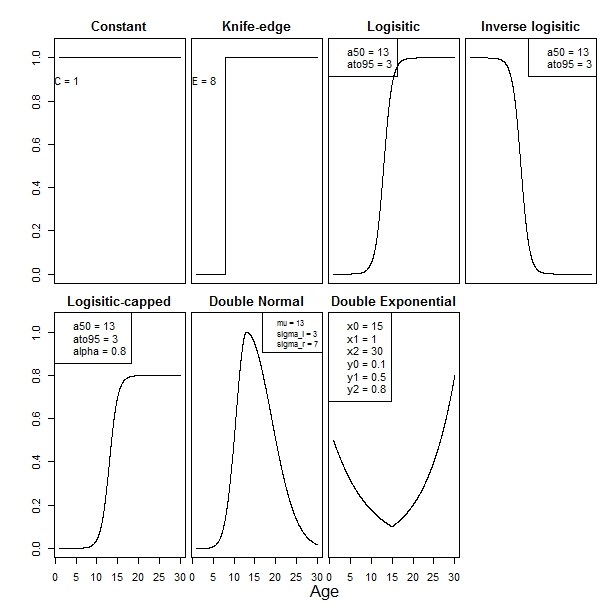
\includegraphics[scale = 0.7]{Figures/Selectivities.jpeg}
	\caption{Examples of the selectivities}
	\label{fig:select examples}
\end{figure}

\subsection{\I{Time-varying Parameter}}\label{sec:TimeVarying} \STATUS{Untested}

Any parameter can be varied annually for blocks of years or in specific years within the model run. For years that are not specified, the parameter will default to the input, or if in an iterative state such as estimation mode, the value being trialled at that iteration. The value used in the configuration file, input parameter file, or trialled value during estimation should be applied during initialisation phases.

Method types for a time-varying parameter are:

\begin{itemize}
\item \subcommand{constant},
\item \subcommand{random\_walk},
\item \subcommand{exogenous},
\item \subcommand{linear},
\item \subcommand{annual\_shift}, and
\item \subcommand{random\_draw}.
\end{itemize}

This option allows for a parameter to be fixed in a year, or be the result of a deterministic or stochastic equation. \textbf{Note:} the stochastic time-varying functionality was added for simulation purposes. \textbf{It has not been tested in an estimation context.}

To implement hierarchical models, the prior parameter values need to be estimated using hyperpriors. To implement a hierarchical model using the time-varying functionality, use MCMC estimation as a way to calculate the integral which is required to obtain unbiased estimates. In an MCMC context, a Gibbs sampler is assumed. That is, every draw is from a conditional distribution and so every draw is a candidate value. \TODO{review}

When allowing removals with annually varying catchabilities, selectivities, and/or other model components, simulated observations more closely model real data. Implementing time-varying parameters also allows for mean or location parameters of selectivities to change between years based on an linked variable.

An example of this is in the New Zealand hoki stock assessment where the $\mu$ and $a_{50}$ parameters are allowed to shift depending on when the fishing season occurs. Descriptive analysis showed that when fishing was earlier relative to other years smaller fish were caught and vice versa. This can be shown in the Examples/2stock directory, implemented at line: \texttt{382} in the \texttt{population.csl2} file. [Craig to edit]

\subsubsection[Constant (year blocks)]{\argument{constant}}\index{Time-varying Parameters!Constant}\label{sec:TimeVarying-Constant}

This option allows a parameter to have an different value during specified years than the rest of the model run. This value can be estimated.

To allow survey catchability to be different in the year block 1975 to 1988 from the rest of the series we write:

{\small{\begin{verbatim}
		@time_varying q_time_var
		type          constant
		parameter     catchability[survey_q].q
		years         1975:1988
		values        0.001      #same for all years
		\end{verbatim}}}

To estimate catchability for 1975 and 1976, use the following:

{\small{\begin{verbatim}
		@estimate q_time_var
		type uniform   #prior
		parameter time_varying[q_time_var].values{1975:1976}
		lower_bound 1e-6 1e-6
		upper_bound 2     2
		\end{verbatim}}}

To make the catchability be same over the year block we need to estimate it for one year (say 1975) and use the \textit{same} subcommand to make the others take the same value

{\small{\begin{verbatim}
		@estimate q_time_var
		type uniform
		parameter time_varying[q_time_var].values{1975}
		same      time_varying[q_time_var].values{1976:1988}
		lower_bound 1e-6
		upper_bound 2
		\end{verbatim}}}

\textbf{Caution}: do not estimate both the actual parameter and its time-varying counterpart, as the time-varying value will overwrite the actual parameter making the actual value unidentifiable. [Craig to edit]

\subsubsection[Random Walk]{\argument{random\_walk}}\index{Time-varying Parameters!Random Walk}\label{sec:TimeVarying-RandomWalk}

A random deviate drawn from a standard normal distribution is added to the previous year's value. This option has an estimable parameter $\sigma_p$ for each time-varying parameter $p$. For reproducible modelling when using stochastic functionality, set the random seed (see Section~\ref{sec:CommandLineArguments}).

{\small{\begin{verbatim}
		@time_varying q_time_var
		type          random_walk
		parameter     catchability[survey_q].q
		distribution  normal
		mean          0
		sigma         3
		\end{verbatim}}}

If the \texttt{parameter} specified in the \command{time\_varying} block is associated with an \command{estimate} block, then the parameter is constrained to stay within the lower and upper bounds of the \command{estimate} block.

\textbf{WARNING:} if the parameter does not have an associated \command{estimate} block then there is no safeguard against the application of a random deviate resulting in parameter values which cause the model to fail, i.e., generates NA or INF values. To avoid this, specify an \command{estimate} block even though the parameter is not actually being estimated; see the example syntax below.

A constraint whilst using this functionality is that a parameter cannot be less than 0.0. If it is then \CNAME\ sets it equal to 0.01.

{\small{\begin{verbatim}
		@estimate survey_q_est
		type      uniform
		parameter catchability[survey_q].q
		lower_bound 1e-6
		upper_bound 10
		\end{verbatim}}}

This configuration will insure the random walk time-varying process will set the any new candidate values within the lower and upper bound of the \command{estimate} block.

\TODO{Syntax abuse: now overloaded many parameters with just one universal one?}

\subsubsection[Annual shift]{\argument{annual\_shift}}\index{Time-varying Parameters!Annual shift} \label{sec:TimeVarying-AnnualShift}

A parameter generated in year $y$ ($\theta'_y$) depends on the value specified by the user ($\theta_y$) along with three coefficients $a$, $b$, and $c$

\begin{equation}
\bar{\theta}_y = \frac{\sum_{y}^Y\theta_y}{Y}
\end{equation}

\begin{equation}
\theta'_y = a \bar{\theta}_y + b\bar{\theta}_y^{2} + c\bar{\theta}_y^{3}
\end{equation}

\subsubsection[Exogenous]{\argument{exogenous}}\index{Time-varying Parameters!Exogenous}\label{sec:TimeVarying-Exogenous}

Parameters are shifted based on an exogenous variable. An example of this is an exploitation selectivity parameters that may vary between years based on known changes in exploitation behaviour such as season, start time, and average depth of exploitation.

\begin{equation}
\delta_y = a(E_y - \bar{E})
\end{equation}

\begin{equation}
\theta'_y = \theta_y + \delta_y
\end{equation}

where $\delta_y$ is the shift or deviation in parameter $\theta_y$ in year $y$ to generate the new parameter value in year $y$ ($\theta'_y$). $a$ is an estimable shift parameter, $E$ is the exogenous variable, and $E_y$ is the value of this variable in year $y$. For more information readers can see \cite{francis_03}.

\subsection{\I{Equation Parser}\label{sec:eq_parser}} \STATUS{Untested}

\CNAME\ has an equation parser, which is currently implemented in Projections (Section~\ref{sec:Project}), Derived quantities (Section~\ref{sec:DerivedQuantity}), and Reports (Section~\ref{sec:Report}).

Examples of syntax for implementing the equation parser are below. For more information on the parser, see \url{https://github.com/nickgammon/parser/blob/master/parser.cpp}

{\small{\begin{verbatim}
		equation process[Recruitment].r0 * 2 #double the recruitment
\end{verbatim}}}

mathematical functions such as \texttt{sqrt()}, \texttt{log()},  \texttt{exp()},  \texttt{cos()}, \texttt{sin()}, and \texttt{tan()} can be used

{\small{\begin{verbatim}
		equation sqrt(process[Recruitment].r0)
\end{verbatim}}}

exponents can be used with \texttt{pow()}

{\small{\begin{verbatim}
		equation pow(2, 3)
\end{verbatim}}}

the absolute value of an equation using \texttt{abs()}

{\small{\begin{verbatim}
		equation abs(sqrt(process[Recruitment].r0) * 1.33)
\end{verbatim}}}

\texttt{if-else} statements can be used

{\small{\begin{verbatim}
		equation if(process[Recruitment].r0 > 23, 44, 55)
		## if R0 is greater than 23 return 44 else return 55
\end{verbatim}}}

\texttt{if-else} statements can also be linked, more complex syntax

{\small{\begin{verbatim}
# if R0 > 23 return 44
# else if R0 < 23 & r0 > 10 return 55
equation if(process[Recruitment].r0 > 23, 44,
         if(process[Recruitment].r0 > 10, 55, 66))
else R0 must be less than 10 return 66
\end{verbatim}}}

Only single values can be referenced, so an equation cannot be applied to a vector, e.g., \subcommand{process[Recruit].ycs\_values\{1974:1980\}} cannot be referenced. More information on which parameters can be included in the equation parser is available (Section~\ref{sec:syntax}). Any subcommand that has a \texttt{type estimable} could be referenced with the equation parser.

\textbf{Note:} the equation parser will not catch all user configuration errors, such as checking whether a parameter that exists in the system has been populated when it is required.

For example, the wrong year could be misspecified in the case of removals in year $y$ which is based on the state of the population in year $y-1$

{\small{\begin{verbatim}
		parameter process[removals].catch
		year 2015
		equation derived_quantity[percent_b0].values{2020}
\end{verbatim}}}

This example is a valid equation but it will have nonsensical results, since a value for 2020 is to be calculated using values for 2015. Although the equation parser adds flexibility, it is easy to misspecify equations.

\subsection{\I{Specifying projections}}\label{sec:Project} \STATUS{Untested}

Given a set of estimated parameter values from a \textit{-e} or a MCMC run,
the model can be projected. Projection years are after the model run years, and are defined in the \command{model} command block using the \subcommand{final\_projection\_year} subcommand, i.e., projection years are \subcommand{final\_year + 1} through to \subcommand{final\_projection\_year}.

Parameter values for the projected years can be specified in a stochastic way or fixed at some value (the default is the estimated value if the parameter is not time-varying) and these are specified in the \command{project} block,

{\small{\begin{verbatim}

@project Future_ycs  # label
type       lognormal_empirical  # which method to use
parameter  process[Recruitment].ycs_values
years      2012:2016
multiplier 1
... # any other parameters
\end{verbatim}}}

The subcommands \subcommand{years} and \subcommand{parameter} are common to all projection methods. Subcommand \subcommand{years} specifies the years to apply the new values to for the parameter in \subcommand{parameter}. Note that the years can be before the \textit{final\_year}, e.g., it is normal to vary the last few recruitment multipliers (YCS) in a projection run because they are usually poorly estimated or they have been set to 1.  The argument \argument{multiplier} is a constant which is multiplied with the projected value after it has been generated. The \subcommand{type} subcommand gives the method to use to generate new parameter values.

\CNAME\ allows any estimable parameter to be specified in a \command{project} block and then varied from the estimated value in a projection. The available projection types for these parameters include:

\begin{itemize}
	\item constant
	\item lognormal
	\item empirical-lognormal
	\item empirical re-sampling
	\item user-defined
\end{itemize}

\CNAME\ has no default projection properties for parameters that are specified by year, e.g., recruitment multiplier parameters, time-varying parameters, and as a special case, future catches. For these, projections  must have a \command{project} command block. For example, \CNAME\ will produce errors if run in projection mode without a \command{project} block for the \subcommand{ycs\_values} parameter being specified.

DEPRECATED: \textbf{Note for the year class parameters:} the definition of year applies to the \argument{ycs\_years}, not the model years. As defined in Section~
\ifAgeBased
\ref{sec:Process-RecruitmentBevertonHolt}
\else
\ref{sec:Process-Length-RecruitmentBevertonHolt}
\fi, \argument{ycs\_years} are offset between the time of spawning and when individuals are added to the partition.

Future catches are also specified in a \command{project} block, one for each fishery (see \ref{sec:Project-Catch} for examples). Here, a fishery is reference in the \textit{parameter} subcommand with the \textit{method\_} fragment to identify it,

 \textit{process[block label].method\_$[$fisheries label$]$},

For a process called \textit{Fishing} that has three fisheries defined, it would be \textit{process[Fishing].method\_pot} to specify the fishery labelled \textit{pot}.

The \CNAME\ command to run the model in projection mode is \texttt{Casal2 -f 1}. \TODO{review; NOT IN MANUAL OR ELSEWHERE]} This functionality allows for the exploration of many scenarios with a single set of parameters. The number of projections should be greater than 1 only if applying a projection type that is stochastic.

The \texttt{-{}-tabular} flag should be used when running projections after a Bayesian analysis. This option will output a tabular report (see Section~\ref{sec:Tabular}) which can then be analysed in \R.

An example of the command line evocation is

\textit{casal2 -f 1 -i mcmc.txt --tabular $>$ projection.out.txt}

where \textit{mcmc.txt} is output from a MCMC run, one parameter set per row, which will give one projection per row, and \textit{projection.out.txt} will contain one row for each MCMC run in each of the reports specified in (usually) the \textit{Report.csl2} file (quantities as specified in the \textit{Report.csl2} file).

For a projection run in \CNAME, the model is initialised and run through the model years from \argument{start\_year} to \argument{final\_year}. During this run mode \CNAME\ stores all parameter values so that projection classes can allow parameters before \subcommand{final\_year} to be projected. The model then is re-run from \argument{start\_year} to \argument{projection\_final\_year}, where any parameter can either be fixed or drawn from a stochastic distribution or process.


\subsubsection{\I{Projection methods}\label{sec:ProjectionMethods}}

This section lists all the projections classes available, their functionality, and an example of the syntax.

\paragraph[Constant]{The constant projection type, \argument{constant}}\index{Projections!Constant}\label{sec:Project-Constant}

A parameter can either be fixed during all projection years or specified individually for each projection year. This is a deterministic assumption, where the parameter is assumed to be known without error during projection years.

{\small{\begin{verbatim}
		@project Future_ycs
		type      constant
		parameter process[Recruitment].ycs_values
		years     2012:2016
		values    1 2 1 2 0.5  #"values 3" means all years use 3
		multiplier 1
		\end{verbatim}}}


\paragraph[Multiple Values]{The multiple values projection type, \argument{multiple\_values}}\index{Project-MultipleValues}\label{sec:Project-MultipleValues}

Users can specify a set of values for each projection year for each row in the \texttt{-i} or \texttt{-I} file using the \subcommand{multiple\_values} projection class. This gives users flexibility in specifying a range of bespoke values during projections and including uncertainty in the projected values. See below for an example on how to configure this class.

{\small{\begin{verbatim}
@project future_disease_rates
type multiple_values
parameter process[dtransition].proportions{disease}  
years 2024:2026
table values
2024 2025 2026
0.1 0.2 0.3
0.3 0.4 0.5
end_table
\end{verbatim}}}

\paragraph[Empirical sampling]{Sampling from a range of years, type  \argument{empirical\_sampling}}\index{Projections!Empirical sampling}\label{sec:Project-EmpiricalSampling}

Parameters that have time components associated with them can be sampled uniformly with replacement over a range of years and used as values for the projected years. The year range to sample from is between \argument{start\_year} and \argument{final\_year}:

{\small{\begin{verbatim}
		@project   Future_ycs
		type       empirical_sampling
		parameter  process[Recruitment].standardised_recruitment_multipliers
		years     2012:2016
		start_year 1988     # re-sample from estimated values
		final_year 2008     # from 1988 to 2008 inclusive
		multiplier 1
		\end{verbatim}}}

\paragraph[Lognormal]{Sampling from a lognormal distribution, type  \argument{lognormal}}\index{Projections!Lognormal}\label{sec:Project-LogNormal} \STATUS{Untested}

The parameters are drawn from a Gaussian distribution in log space and exponentiated  to result in the lognormal distribution

\begin{equation}\label{eq:lognormal}
X_p = exp(\epsilon_p - \sigma^2 / 2)
\end{equation}

where $\epsilon_p\stackrel{iid}{\sim}N(\mu,\sigma)$ and $X_p$ is the projected value for parameter $X$, and $\mu$ and $\sigma$ are the mean and standard deviation on the log scale.

An example of applying this process to draw future year class parameters from a lognormal distribution with mean 1 and standard deviation 0.8

{\small{\begin{verbatim}
		@project Future_ycs
		type     lognormal
		parameter process[Recruitment].ycs_values
		years     2012:2016
		mean      0     #mean 1 on un-transformed scale
		sigma     0.8   # log scale
		multiplier 1
		\end{verbatim}}}

\paragraph[Lognormal-Empirical]{Sampling from a lognormal distribution where the  variance is estimated from values over a specified year range, type  \argument{lognormal\_empirical} }\index{Projections!Lognormal-Empirical}\label{sec:Project-LogNormalEmpirical} \STATUS{Untested}

This method applies a lognormal draw as in the \argument{LogNormal} method above and specifies a year range from which the standard deviation of the distribution is calculated. Then equation~\eqref{eq:lognormal} is used to generate future values with a specified $\mu$ and empirically calculated $\sigma$,

{\small{\begin{verbatim}
		@project Future_ycs
		type      lognormal_empirical
		parameter process[Recruitment].ycs_values
		years     2012:2016
		mean      0
		start_year 1988   # range of years to take the
		final_year 2008   # values for \math{\sigma}
		multiplier 1
		\end{verbatim}}}

%\paragraph[User Defined]{Sample from a user-defined function, \argument{user\_defined}}\index{Projections!User Defined}\label{sec:Project-UserDefined} \STATUS{Untested}

%This method uses the equation parser to calculate the values to use in the projection. This was set up to define and apply harvest control rules (e.g., apply a management action such as changing catch limits based on the current or previous state).

%In fisheries models, this option can be used to calculate the projected catch based on an exploitation rate multiplied by the vulnerable biomass, where the exploitation rate is based on a rule (Figure~\ref{fig:HCR}).

%\begin{figure}[!h]
%	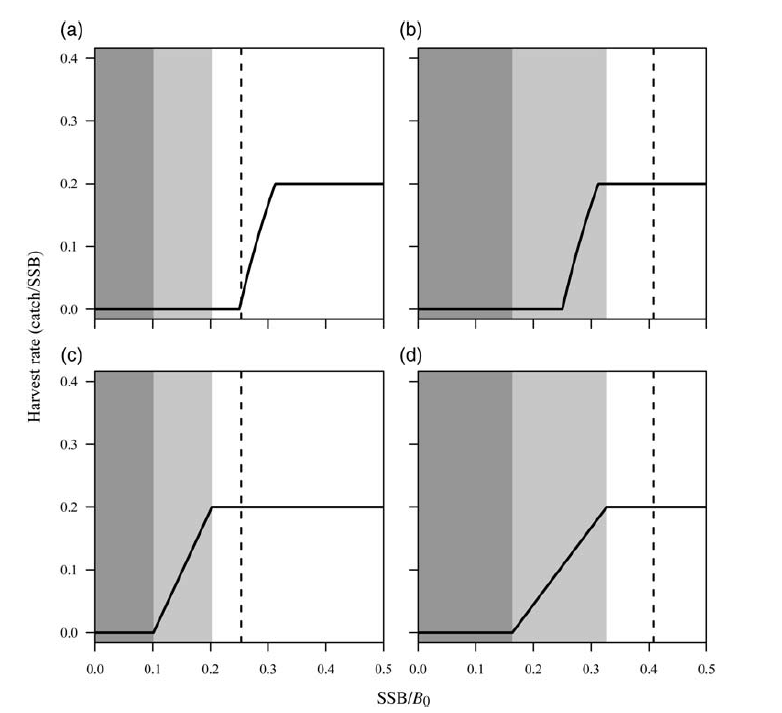
\includegraphics[scale=0.9]{Figures/HarvestControlRules.png}
%	\caption{\textbf{Examples of control rules based on current stock status.}}
%	\label{fig:HCR}
%\end{figure}

%\pagebreak
%{\small{\begin{verbatim}
%		@project HCR_2015
%		type       user_defined
%		parameter process[Instantaneous_Mortality].method_Sub_Ant_F
%		years 2015
%		equation if(derived_quantity[SSB].values{2014} / process[Recruitment].b0 <= 0.1, 0.0,
%		if(derived_quantity[SSB].values{2014} / process[Recruitment].b0 > 0.1 &&
%		derived_quantity[SSB].values{2014} / process[Recruitment].b0 < 0.2,
%		derived_quantity[SSB].values{2014} * derived_quantity[SSB].values{2014}
%		/ process[Recruitment].b0,
%		derived_quantity[SSB].values{2014} * 0.2))
%		\end{verbatim}}}

%Care should be taken when writing user-defined equations. The above equation is: if $\%B_{2014} \leq 0.1$ then set next year's catch to 0.0, else if $\%B_{2014} > 0.1 \text{ } \& \text{ } \%B_{2014} \leq 0.2$ then set next year's catch equal to $\%B_{2014} \times SSB_{2014}$, else set next year's catch to $0.2 SSB_{2014}$.

\paragraph[Catches]{Specifying catch for projections }\index{Projections!Catches}\label{sec:Project-Catch}

Catches are unique in that they are known inputs in a table format. For example, to project catches that are in a table

{\small{\begin{verbatim}
# fishing process
@process Fishing
type mortality_instantaneous_retained
m 0.17*6  #0.17    #testing at old values
time_step_proportions 1
relative_m_by_age One*6   #for age based M
categories *
table catches
year	FishingLine	FishingPot	Recreation
1900	0	0	0
1901	13.2	0	22.9
1902	26.4	0	23.5
1903	39.6	0	24
end_table

# projection block
@project future_catch
type      constant
parameter process[Fishing].method_fishingpot
years     2020:2029
values    4000
\end{verbatim}}}

This uses the syntax \texttt{block\_type[block\_label].method\_fishinglabel}. \textbf{Note:} the fishing label which is defined in the table needs to be lower case form in the \command{projection} block. Notice the use of \textit{method\_} syntax to identify the right fishery.
